\chapter{Introdução}

\section{Introdução}

Este presente trabalho tem como objectivo demonstrar a implementação de um sistema de gestão de receitas e ingredientes para um Chefe de Restaurante.

Sendo este uma \textit{fork} de duas tarefas de quatro totais demonstradas num trabalho prévio, o qual no capitulo seguinte está uma renderização do mesmo.

\section{Estrutura deste Relatório}

Este relatório está organizado da seguinte forma: Introdução, Analise do Sistema (onde se usa o trabalho de analise da época normal, o qual está bom e saturado de boa informação), Inicio e caracterização do Projecto, Base de dados, Implementação da API, Implementação da WebApp, Testes, Conclusão.

\section{Análise do Sistema}

A análise deste sistema foi feita em época normal, como tal devo repetir palavra por palavra o que foi dito, ou seja, colocar o exacto mesmo conteúdo nas secções seguintes.

O objectivo geral deste trabalho é a criação de um website que permita o acesso aos clientes e funcionários do restaurante aos menus disponíveis na ementa, mesas disponíveis, reservas no restaurante, gestão do stock de alimentos.

Para suportar o website, é necessária uma base de dados que seja capaz de guardar todas as informações sobre os funcionários, ementas, stock no restaurante e organizada de forma que o relacionamento entre as entidades seja bom, isto porque, se existir uma base de dados bem-criada, não existira redundância logo ocorrerá um aumento de eficiência.

O sistema será criado com intenção que qualquer restaurante interessado possa utilizar, uma vez que, graças a ele será possível uma melhor gestão dos acontecimentos dentro do restaurante, assim como de um melhor controlo dos stocks e mais facilidade para os clientes de consultar o cardápio e reservar mesas.

Assim sendo, pretende-se criar um sistema que permita o gestão de restaurantes (stocks, receitas, etc.).

Para distinguir entre utilizadores e funcionários, cada um terá permissões diferentes dentro website possibilitando algumas opções ou desabilitando outras.

O presente relatório encontra-se organizado na seguinte forma: na secção 2 descreve-se a fase de análise do projecto; na secção 3 descreve-se a fase de desenho, mais nomeadamente a construção de cenários de utilização e o desenho do protótipo; na secção 4 é descrito conclusões relativas à elaboração do trabalho.

\subsection{Análise}

Na fase de análise do projecto foram recolhidas diversas informações sobre o sistema a implementar.

Essas informações serviram como base para a construção do projecto, isto é, das tarefas disponibilizadas ao utilizador e também algumas opções mais tarde utilizadas na fase de desenho

\subsection{Caracterização dos Actores}

Foram desenvolvidas três personas para ajudar na caracterização dos actores, uma para cada tipo de utilizador. Em seguida apresentam-se as personas criadas:

\begin{itemize}
    \item \textbf{Raul Joaquim (Funcionário):} O Raul tem 32 anos, é da zona o Porto, mas actualmente está a viver em Albufeira com a sua mulher e 2 filhos, onde é funcionário do maior restaurante da localidade desde os seus 24 anos. O Raul terminou o ensino secundário ainda no Porto, mas mais tarde decidiu tirar um curso de restauração em Albufeira, onde acabou por ficar a viver e trabalhar. Para alem do restaurante onde o Raul está neste momento, ele também teve várias experiências como funcionário de vários cafés e restaurantes menores anteriormente, tendo assim uma vasta carreira profissional na área. Porém o Raul nunca teve o hábito de usar muitas tecnologias frequentemente, apenas o mínimo como navegar em websites para consultar alguns produtos ou fazer encomendas. Quer isto dizer que o Raul tem apenas os conhecimentos básicos no uso de websites
    \item \textbf{Ivone Silva (Gerente):} A Ivone tem 43 anos, nasceu e vive na zona de Lisboa com o seu marido á cerca de 12 anos e com as suas duas filhas. A Ivone actualmente trabalha como gerente de vários restaurantes, uma vez que todos pertencem á mesma empresa, há 11 anos. Acabou o secundário com uma média elevada na escola mais prestigiada de Lisboa, e neste momento já se encontra licenciada em Engenharia Informática, Gestão de Empresas e Restauração, Porem começou a trabalhar como gerente logo quando terminou os dois primeiros cursos mencionados, actualmente tem um cargo bastante importante na empresa uma vez que possui um grande à vontade em fazer um pouco de tudo dentro da mesma. Sendo assim, a Ivone entende perfeitamente como utilizar e aceder a websites uma vez que o faz no seu dia a dia, dentro e fora do trabalho
    \item \textbf{João Miguel (Cliente):} O João Miguel tem 18 anos, nasceu e vive em Beja com os seus pais e irmão mais novo e é estudante na Escola Secundária D. Manuel I em Beja, como o João Miguel concretizou recentemente os seus 18 anos ele pretendia realizar uma festa de anos com os seus amigos e família no restaurante Milano. O João sempre teve uma enorme paixão por tecnologias em especial vídeo jogos o que lhe fez desenvolver gosto na criação dos mesmos e por isso investigou bastante sobre a maneira como são feitos. O João tem facilidade na utilização de tecnologias recentes, como por exemplo o acesso e uso de websites, pois recorre a estes serviços todos os dias quando investiga mais sobre a criação de jogos
\end{itemize}

\subsection{Diagramas de Casos de Uso}

\begin{figure}[!hbt]
    \centering
    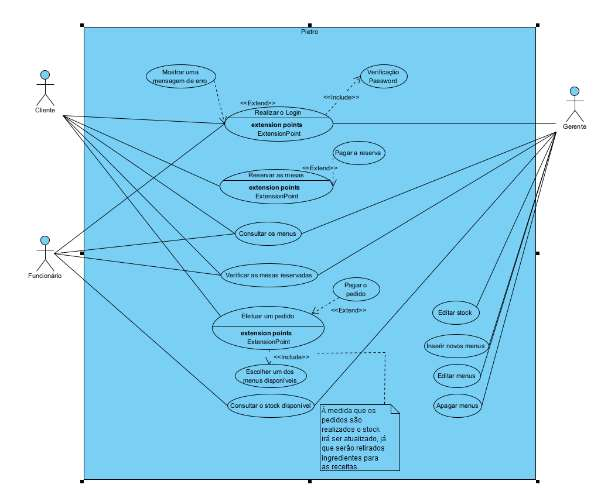
\includegraphics[width=14cm]{Resources/Previous/image-089.jpg}
    \caption{Diagrama de Casos de Uso (UML)}
    
\end{figure}

Quando o diagrama foi terminado, foram analisados os casos de uso e especificamos cada um deles. Para cada um dos casos de uso elaboramos uma breve descrição, definimos as pré e pós condições, o fluxo de eventos entre outras especificações.

De seguida são apresentadas as tabelas com as especificações para cada caso de uso.

\begin{figure}[!hbt]
    \centering
    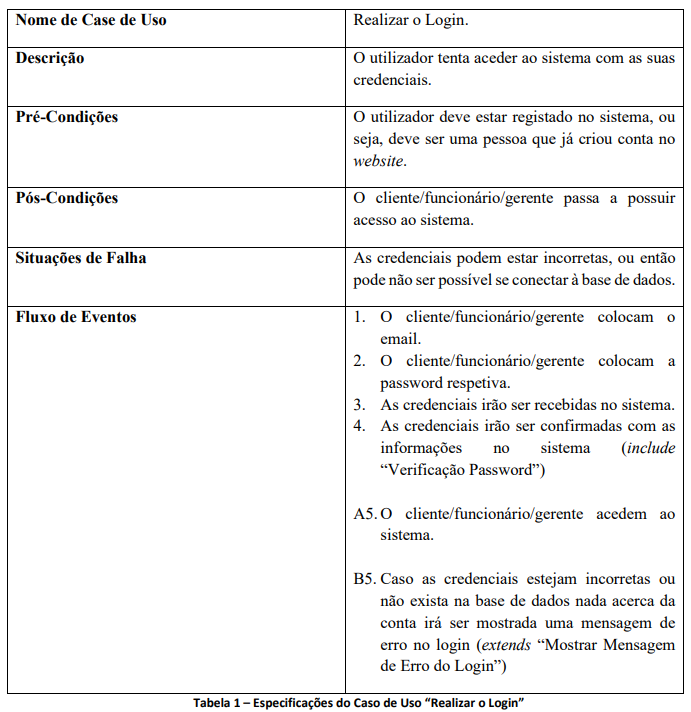
\includegraphics[width=14cm]{Resources/TablesPrintSc/1.png}
    \caption{PrintSc da Tabela 1}
    
\end{figure}
\FloatBarrier
\begin{figure}[!hbt]
    \centering
    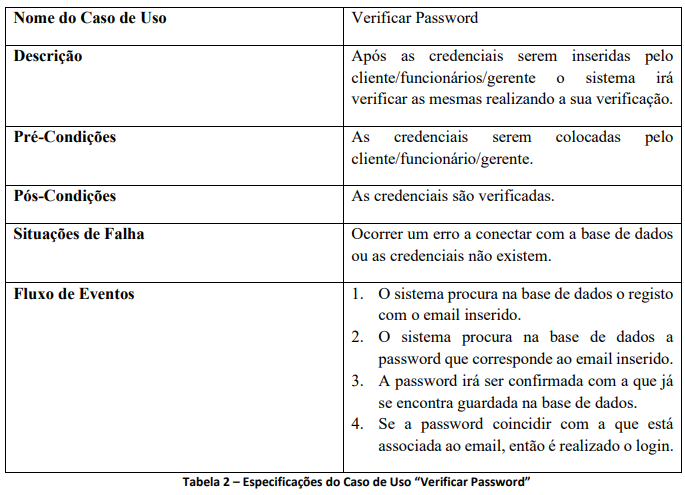
\includegraphics[width=14cm]{Resources/TablesPrintSc/2.png}
    \caption{PrintSc da Tabela 2}
    
\end{figure}
\FloatBarrier
\begin{figure}[!hbt]
    \centering
    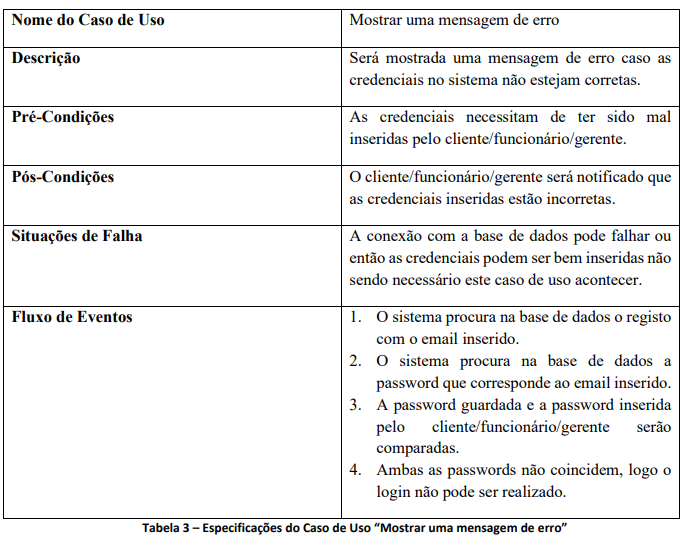
\includegraphics[width=14cm]{Resources/TablesPrintSc/3.png}
    \caption{PrintSc da Tabela 3}
    
\end{figure}
\FloatBarrier
\begin{figure}[!hbt]
    \centering
    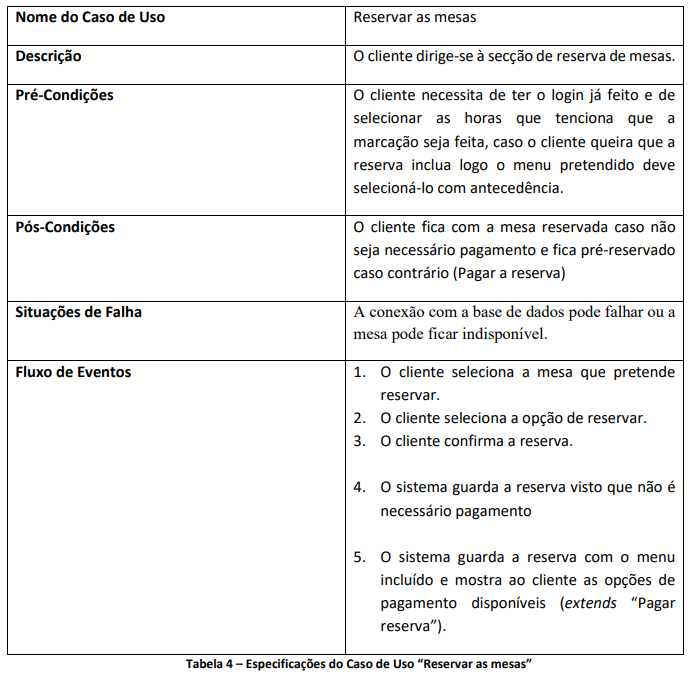
\includegraphics[width=14cm]{Resources/TablesPrintSc/4.png}
    \caption{PrintSc da Tabela 4}
    
\end{figure}
\FloatBarrier
\begin{figure}[!hbt]
    \centering
    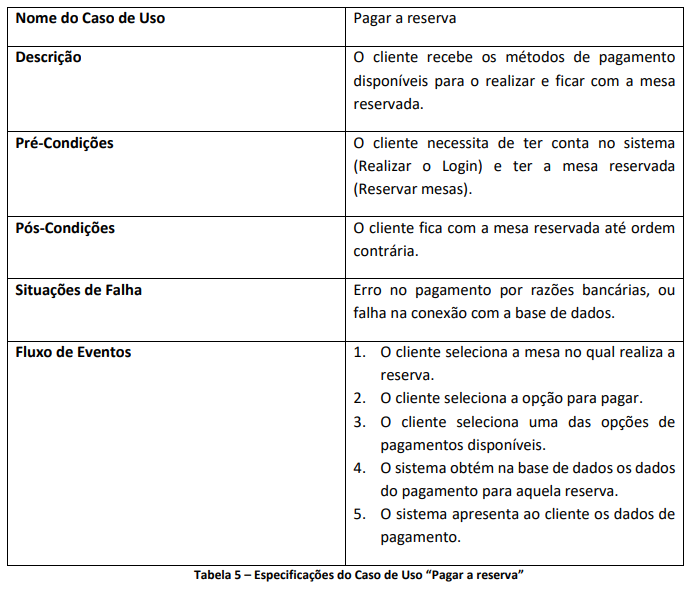
\includegraphics[width=14cm]{Resources/TablesPrintSc/5.png}
    \caption{PrintSc da Tabela 5}
    
\end{figure}
\FloatBarrier
\begin{figure}[!hbt]
    \centering
    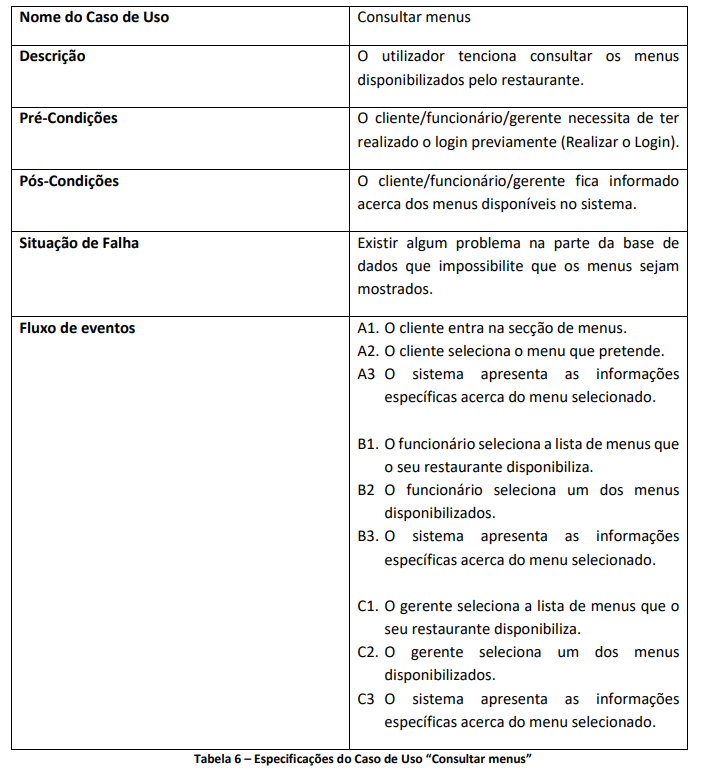
\includegraphics[width=14cm]{Resources/TablesPrintSc/6.png}
    \caption{PrintSc da Tabela 6}
    
\end{figure}
\FloatBarrier
\begin{figure}[!hbt]
    \centering
    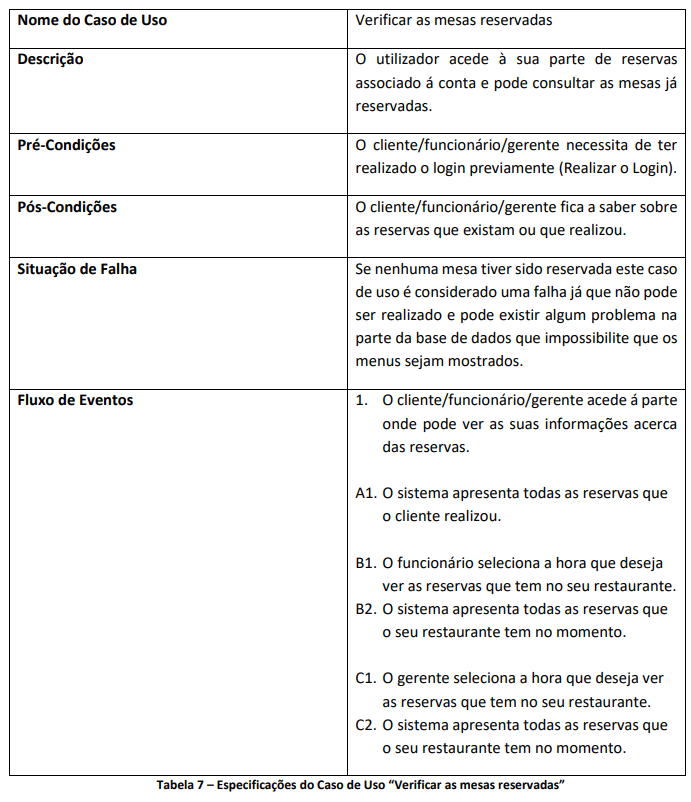
\includegraphics[width=14cm]{Resources/TablesPrintSc/7.png}
    \caption{PrintSc da Tabela 7}
    
\end{figure}
\FloatBarrier
\begin{figure}[!hbt]
    \centering
    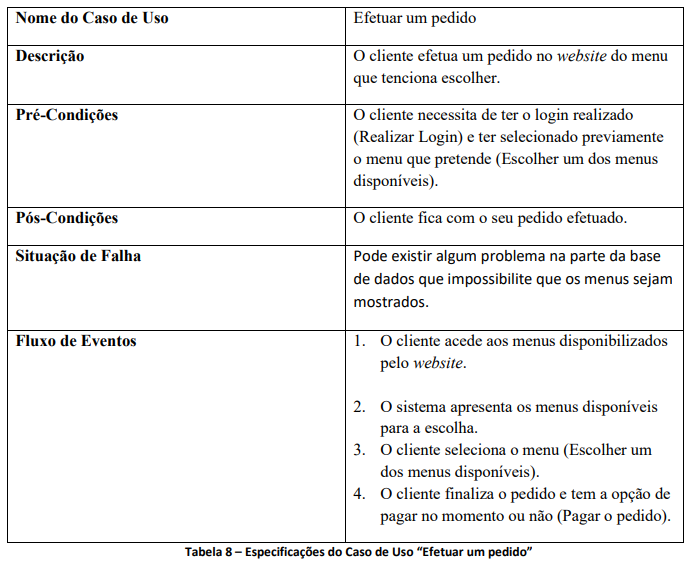
\includegraphics[width=14cm]{Resources/TablesPrintSc/8.png}
    \caption{PrintSc da Tabela 8}
    
\end{figure}
\FloatBarrier
\begin{figure}[!hbt]
    \centering
    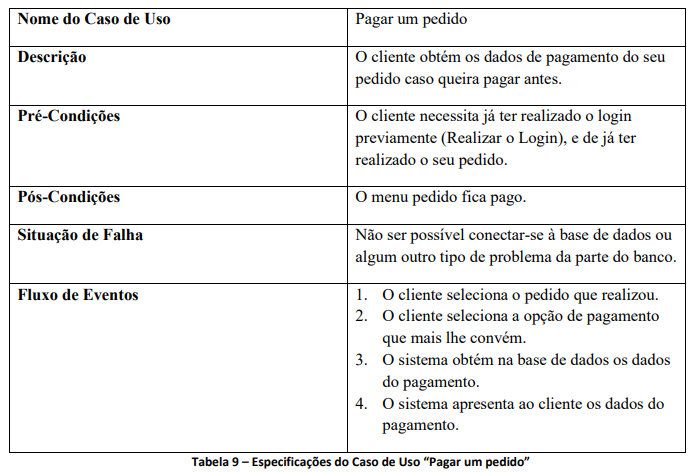
\includegraphics[width=14cm]{Resources/TablesPrintSc/9.png}
    \caption{PrintSc da Tabela 9}
    
\end{figure}
\FloatBarrier
\begin{figure}[!hbt]
    \centering
    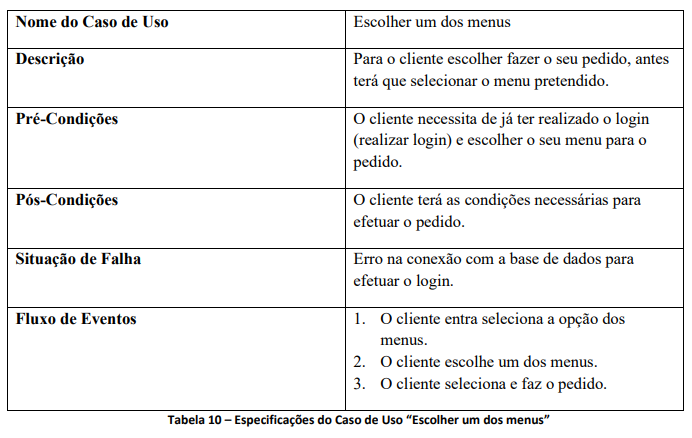
\includegraphics[width=14cm]{Resources/TablesPrintSc/10.png}
    \caption{PrintSc da Tabela 10}
    
\end{figure}
\FloatBarrier
\begin{figure}[!hbt]
    \centering
    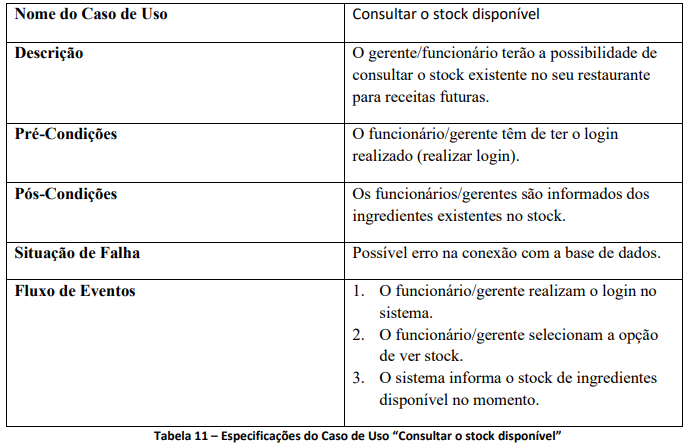
\includegraphics[width=14cm]{Resources/TablesPrintSc/11.png}
    \caption{PrintSc da Tabela 11}
    
\end{figure}
\FloatBarrier
\begin{figure}[!hbt]
    \centering
    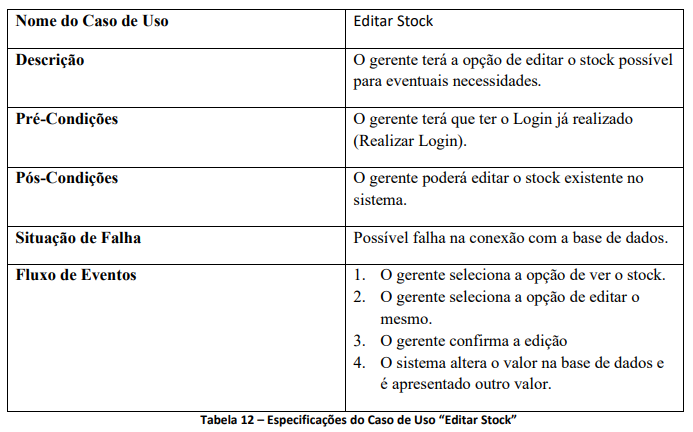
\includegraphics[width=14cm]{Resources/TablesPrintSc/12.png}
    \caption{PrintSc da Tabela 12}
    
\end{figure}
\FloatBarrier
\begin{figure}[!hbt]
    \centering
    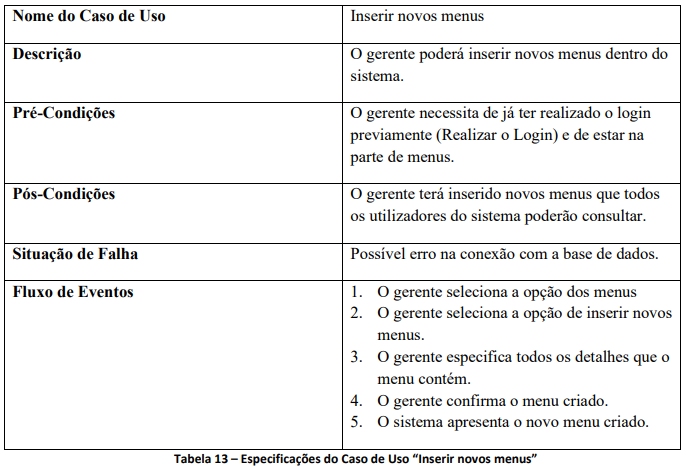
\includegraphics[width=14cm]{Resources/TablesPrintSc/13.png}
    \caption{PrintSc da Tabela 13}
    
\end{figure}
\FloatBarrier
\begin{figure}[!hbt]
    \centering
    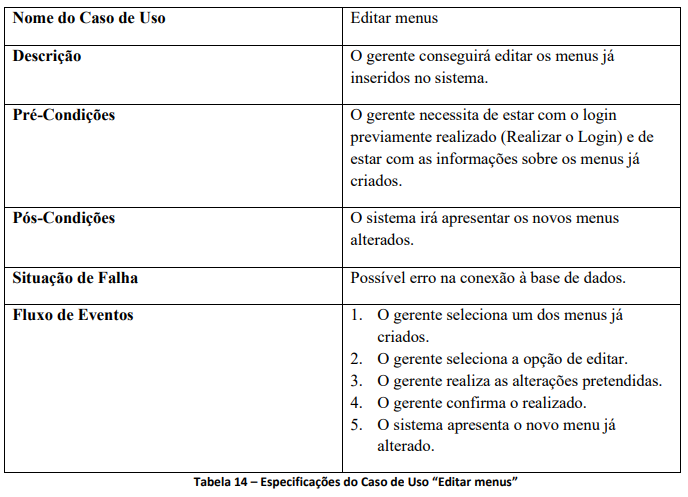
\includegraphics[width=14cm]{Resources/TablesPrintSc/14.png}
    \caption{PrintSc da Tabela 14}
    
\end{figure}
\FloatBarrier
\begin{figure}[!hbt]
    \centering
    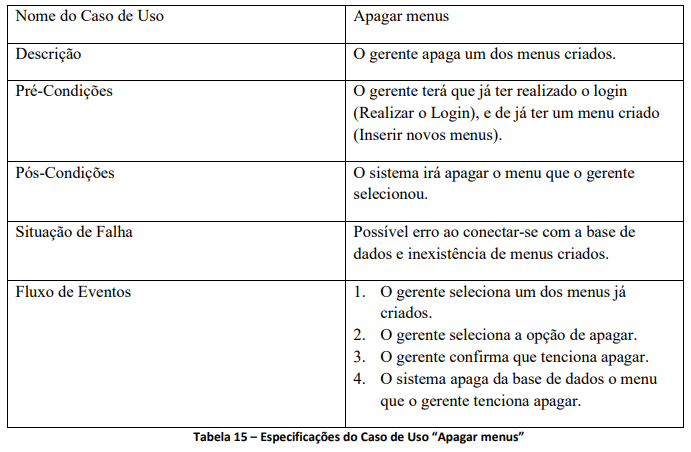
\includegraphics[width=14cm]{Resources/TablesPrintSc/15.png}
    \caption{PrintSc da Tabela 15}
    
\end{figure}
\FloatBarrier

\subsection{Desenho do Sistema}

O desenho inicial do protótipo foi realizado com o intuito de satisfazer todas as necessidades dos diferentes utilizadores na realização das tarefas já apresentadas. O objectivo do desenho foi ser o mais simples possível para que qualquer utilizador consiga utilizar o mesmo, o estilo de desenho que achamos por melhor utilizar foi o Flat Design, uma vez que é dos estilos mais modernos actualmente.


\begin{figure}[!hbt]
    \centering
    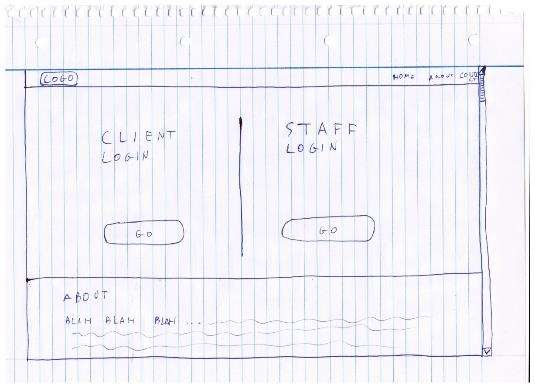
\includegraphics[width=14cm]{Resources/Previous/image-090.jpg}
    \caption{Desenho do Sistema 1}
    
\end{figure}
\FloatBarrier
\begin{figure}[!hbt]
    \centering
    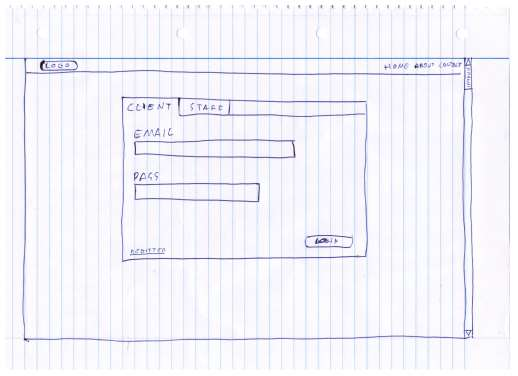
\includegraphics[width=14cm]{Resources/Previous/image-091.jpg}
    \caption{Desenho do Sistema 2}
    
\end{figure}
\FloatBarrier
\begin{figure}[!hbt]
    \centering
    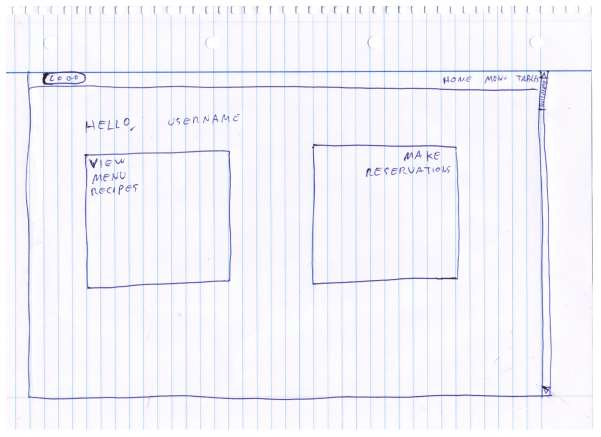
\includegraphics[width=14cm]{Resources/Previous/image-092.jpg}
    \caption{Desenho do Sistema 3}
    
\end{figure}
\FloatBarrier
\begin{figure}[!hbt]
    \centering
    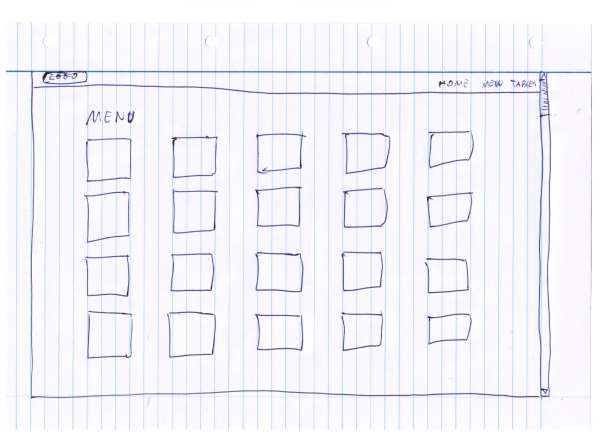
\includegraphics[width=14cm]{Resources/Previous/image-093.jpg}
    \caption{Desenho do Sistema 4}
    
\end{figure}
\FloatBarrier
\begin{figure}[!hbt]
    \centering
    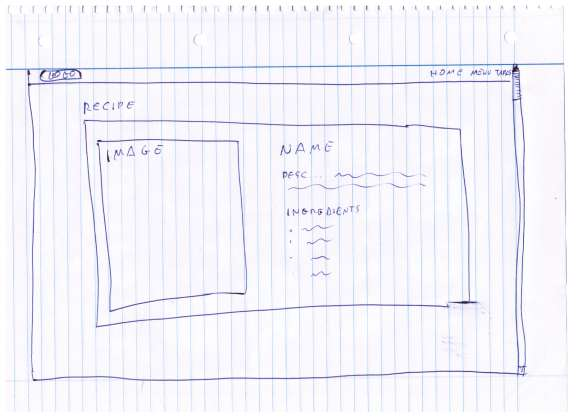
\includegraphics[width=14cm]{Resources/Previous/image-094.jpg}
    \caption{Desenho do Sistema 5}
    
\end{figure}
\FloatBarrier
\begin{figure}[!hbt]
    \centering
    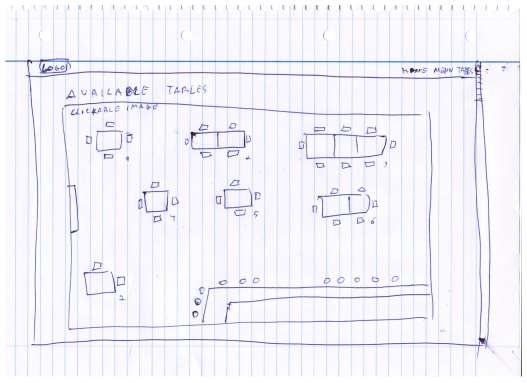
\includegraphics[width=14cm]{Resources/Previous/image-095.jpg}
    \caption{Desenho do Sistema 6}
    
\end{figure}
\FloatBarrier
\begin{figure}[!hbt]
    \centering
    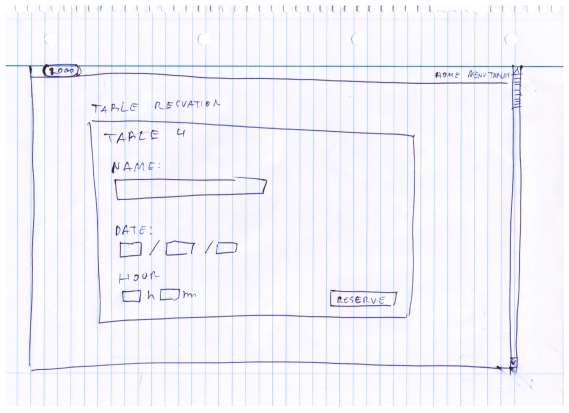
\includegraphics[width=14cm]{Resources/Previous/image-096.jpg}
    \caption{Desenho do Sistema 7}
    
\end{figure}
\FloatBarrier
\begin{figure}[!hbt]
    \centering
    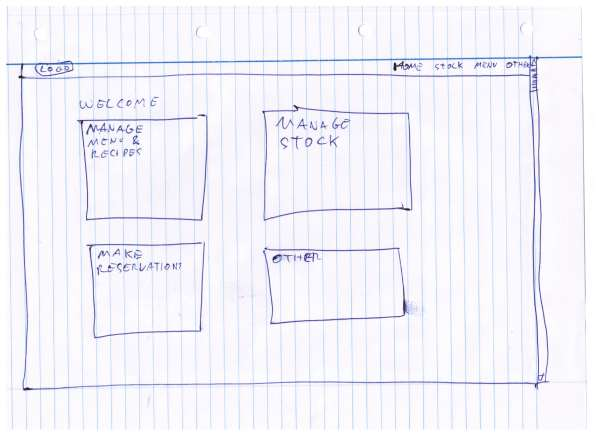
\includegraphics[width=14cm]{Resources/Previous/image-097.jpg}
    \caption{Desenho do Sistema 8}
    
\end{figure}
\FloatBarrier
\begin{figure}[!hbt]
    \centering
    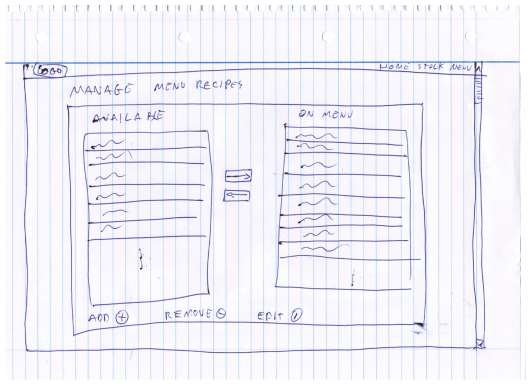
\includegraphics[width=14cm]{Resources/Previous/image-098.jpg}
    \caption{Desenho do Sistema 9}
    
\end{figure}
\FloatBarrier
\begin{figure}[!hbt]
    \centering
    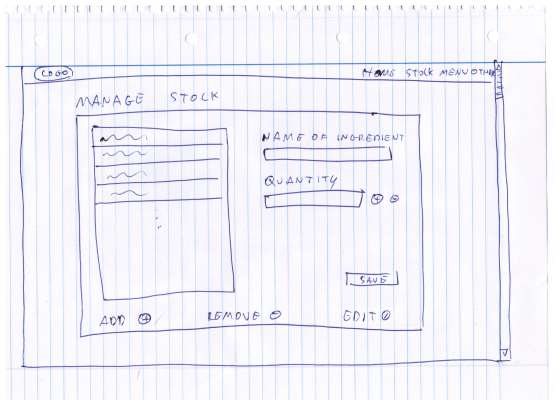
\includegraphics[width=14cm]{Resources/Previous/image-099.jpg}
    \caption{Desenho do Sistema 10}
    
\end{figure}
\FloatBarrier

\subsubsection{\textit{Storyboard}s}

Os \textit{Storyboard}s são desenhos sequenciais que pretendem ilustrar uma certa acção, é uma estratégia bastante útil uma vez que facilita o reconhecimento de erros e incongruências no desenho.

Em seguida são apresentados os \textit{Storyboard}s elaborados.

Caso de uso 1 (Gerir receitas. Adicionar, remover e editar as respectivas receitas de cada menu do cardápio).


\begin{figure}[!hbt]
    \centering
    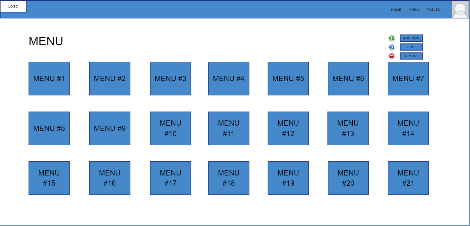
\includegraphics[width=14cm]{Resources/Previous/image-100.png}
    \caption{\textit{Storyboard} para o caso de uso 1}
    
\end{figure}
\FloatBarrier
\begin{figure}[!hbt]
    \centering
    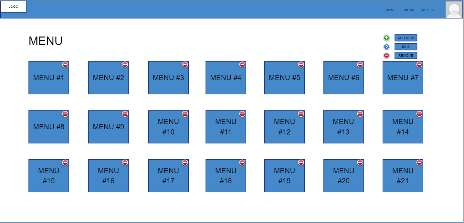
\includegraphics[width=14cm]{Resources/Previous/image-101.jpg}
    \caption{\textit{Storyboard} para o caso de uso 1}
    
\end{figure}
\FloatBarrier
\begin{figure}[!hbt]
    \centering
    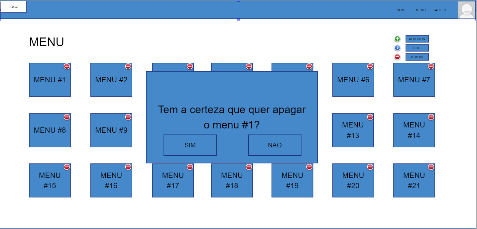
\includegraphics[width=14cm]{Resources/Previous/image-102.png}
    \caption{\textit{Storyboard} para o caso de uso 1}
    
\end{figure}
\FloatBarrier
\begin{figure}[!hbt]
    \centering
    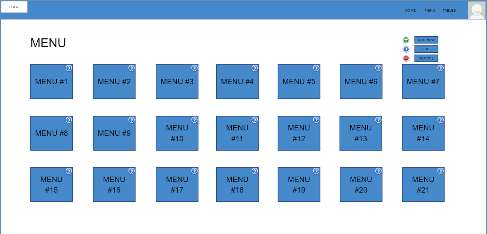
\includegraphics[width=14cm]{Resources/Previous/image-103.jpg}
    \caption{\textit{Storyboard} para o caso de uso 1}
    
\end{figure}
\FloatBarrier
\begin{figure}[!hbt]
    \centering
    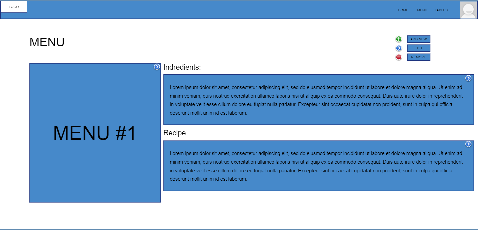
\includegraphics[width=14cm]{Resources/Previous/image-104.png}
    \caption{\textit{Storyboard} para o caso de uso 1}
    
\end{figure}
\FloatBarrier
\begin{figure}[!hbt]
    \centering
    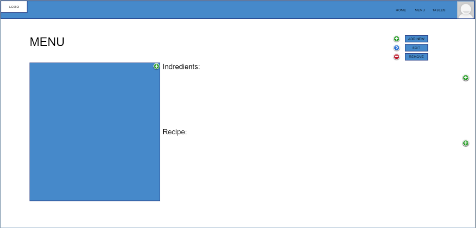
\includegraphics[width=14cm]{Resources/Previous/image-105.png}
    \caption{\textit{Storyboard} para o caso de uso 1}
    
\end{figure}
\FloatBarrier

Caso de uso 2 (Consulta das receitas. O cliente terá a opção de consultar as receitas disponíveis e os ingredientes que cada uma leva assim como alguns outros detalhes que poderão estar presentes.

\begin{figure}[!hbt]
    \centering
    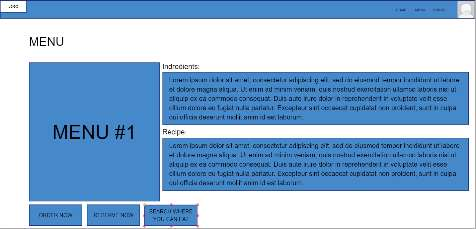
\includegraphics[width=14cm]{Resources/Previous/image-106.jpg}
    \caption{\textit{Storyboard} para o caso de uso 2}
    
\end{figure}
\FloatBarrier

Caso de uso 3 (Sistema de reservas (gerir mesas). Os clientes poderão ter a opção de entrar no sítio web para reservar uma mesa e os pratos que terão em mente.

Á medida que os clientes vão chegando e sentando-se nas devidas mesas, o sistema irá bloquear as mesas correspondentes às que estarão em uso e mais tarde serão desbloqueadas quando os clientes estiverem servidos).

\begin{figure}[!hbt]
    \centering
    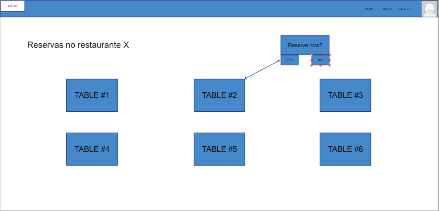
\includegraphics[width=14cm]{Resources/Previous/image-107.png}
    \caption{\textit{Storyboard} para o caso de uso 3}
    
\end{figure}
\FloatBarrier

Caso de uso 4 (Gerir o stock. Ao ser vendido um dos pratos do restaurante, será debitado do stock os ingredientes necessários para realizar a receita. Os funcionários poderão também consultar o stock existente no sistema).

\begin{figure}[!hbt]
    \centering
    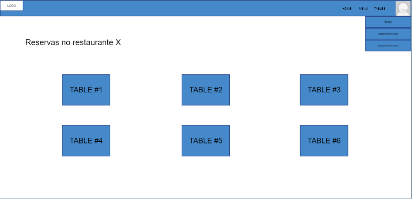
\includegraphics[width=14cm]{Resources/Previous/image-108.png}
    \caption{\textit{Storyboard} para o caso de uso 4}
    
\end{figure}
\FloatBarrier
\begin{figure}[!hbt]
    \centering
    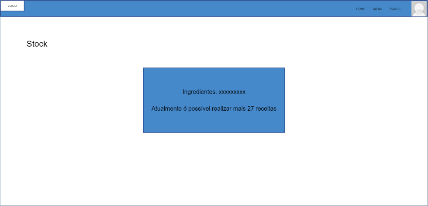
\includegraphics[width=14cm]{Resources/Previous/image-109.png}
    \caption{\textit{Storyboard} para o caso de uso 4}
    
\end{figure}
\FloatBarrier

\subsubsection{\textit{Drafts} das Interfaces 1 e 4}

\begin{figure}[!hbt]
    \centering
    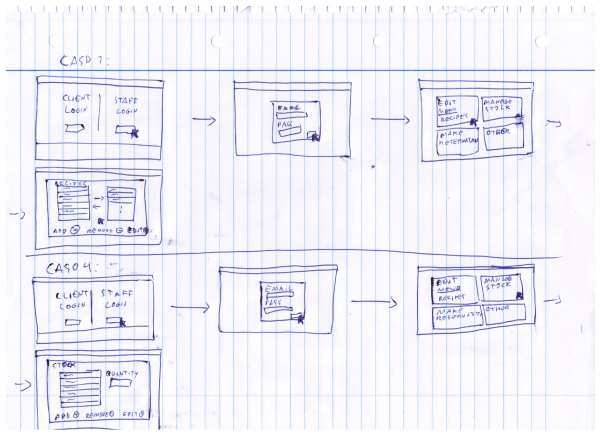
\includegraphics[width=14cm]{Resources/Previous/image-110.jpg}
    \caption{Interfaces para o caso de uso 1 e 4}
    
\end{figure}
\FloatBarrier


\subsubsection{\textit{Drafts} das Interfaces 2 e 3}

\begin{figure}[!hbt]
    \centering
    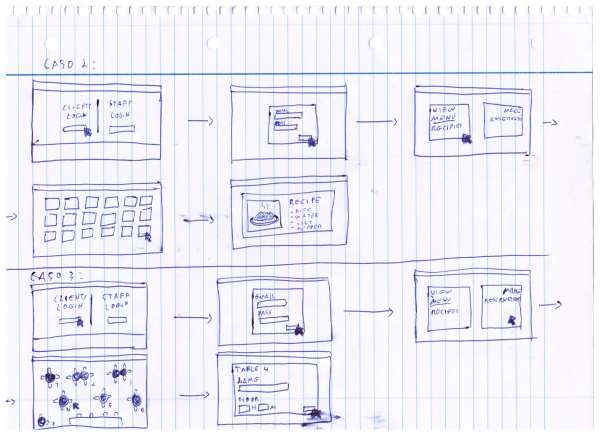
\includegraphics[width=14cm]{Resources/Previous/image-111.jpg}
    \caption{Interfaces para o caso de uso 2 e 3}
    
\end{figure}
\FloatBarrier

\subsection{Modelação da Base de Dados}

De modo que o sistema fosse capaz de armazenar toda a informação necessária, sem criar redundância, identificamos as entidades e as relações estritamente necessárias entre as mesmas no modelo ER. Posteriormente foi desenvolvido o modelo físico baseado no modelo ER.

As imagens dos modelos estão apresentadas logo abaixo.

\subsubsection{Diagrama de Entidade-Relação}

\begin{figure}[!hbt]
    \centering
    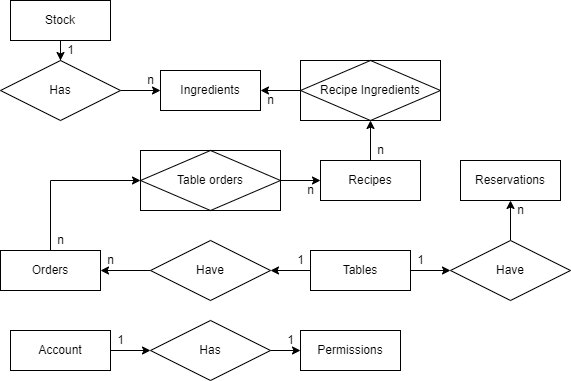
\includegraphics[width=14cm]{Resources/Previous/image-112.png}
    \caption{Diagrama ER}
    
\end{figure}
\FloatBarrier

\subsubsection{Modelo Físico}

\begin{figure}[!hbt]
    \centering
    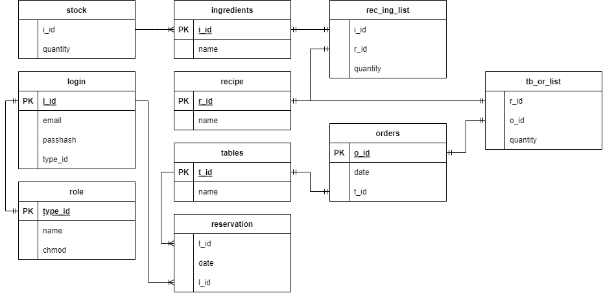
\includegraphics[width=14cm]{Resources/Previous/image-114.png}
    \caption{Modelo Físico}
    
\end{figure}
\FloatBarrier